\chapter{\ifproject%
\ifenglish Project Structure and Methodology\else โครงสร้างและขั้นตอนการทำงาน\fi
\else%
\ifenglish Project Structure\else โครงสร้างของโครงงาน\fi
\fi
}

\enskip \enskip \enskip \enskip \enskip ในบทนี้จะกล่าวถึงการการออกแบบและฟีเจอร์ของแอพพลิเคชั่น นโยบายความเป็นส่วนตัวของผู้ใช้ User interface และการออกแบบฐานข้อมูลของแอพพลิเคชั่น



\makeatletter

% \renewcommand\section{\@startsection {section}{1}{\z@}%
%                                    {13.5ex \@plus -1ex \@minus -.2ex}%
%                                    {2.3ex \@plus.2ex}%
%                                    {\normalfont\large\bfseries}}

\makeatother
%\vspace{2ex}
% \titleformat{\section}{\normalfont\bfseries}{\thesection}{1em}{}
% \titlespacing*{\section}{0pt}{10ex}{0pt}

\section{โครงสร้างของแอพพลิเคชั่น}
\enskip \enskip \enskip \enskip \enskip 
ในเว็บแอพพลิเคชั่นของเราจะมีกลุ่มผู้ใช้อยู่ 2 กลุ่มผู้ใช้คือ ผู้ที่จะออกใบประกาศนียบัตร กับผู้ที่ต้องการตรวจสอบใบประกาศนียบัตร
\subsection{ภาพโดยรวมของเว็บแอพพลิเคชั่น}
\enskip \enskip \enskip \enskip \enskip 
เมื่อผู้ใช้ที่ต้องการจะออกใบประกาศนียบัตรจากเว็บแอพพลิเคชั่นตัวแอพจะรับข้อมูลจากผู้ใช้งานมาแล้วทำการติดต่อกับ
Chaincode  เพื่อ้ก็บข้อมูลลงในblockchain แล้วทำการส่งไปยัง Backend เพื่อทำการ Generate ข้อมูลที่รับมา เพื่อนำไปออกใบประกาศนียบัตร 
ในส่วนของผู้ใช้ที่ต้องการจะตรวจสอบใบประกาศนียบัตรจะทำการแสกน QR CODE แล้วระบบจะแสดงข้อมูลของใบCertificate นั้นที่เก็บไว้เพื่อทำการตรวจสอบ



% \begin{figure}
% \begin{center}
% \includegraphics{800px-Briny_Beach.jpg}
% \end{center}
% \caption[Poem]{The Walrus and the Carpenter}
% \label{fig:walrus}
% \end{figure}

% ~\cite{aiw}
\section{World State Design}
\enskip \enskip \enskip \enskip \enskip
\graphicspath{ {./images/} }
\begin{figure}[htbp]
  \centering 
  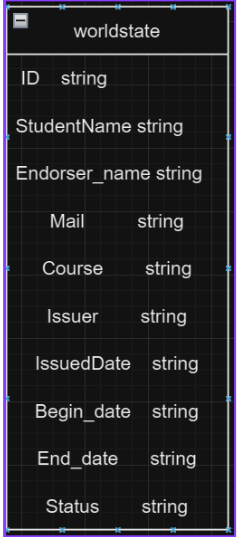
\includegraphics[scale=0.7]{world.png}
  \caption[World State Design]{World State Design}
  \label{fig:World State Design}
\end{figure}
โดยเราจะออกแบบให้เก็บข้อมูลดังนี้
\enskip \enskip \enskip \enskip \enskip
\begin{enumerate}
  \item ID : เก็บว่าเป็นลำดับที่เท่าไหร่
  \item StudentName : ชื่อของนักเรียนที่ผ่านคอร์สนี้
  \item Endorser\_name : ชื่อของคนยืนยัน
  \item Mail : E-Mail ของนักเรียน
  \item Course : ชื่อของคอร์สนี้
  \item Issuer : ชื่อของคนออกใบ Certificate นี้
  \item IssuerDate : วันที่ออกใบ Certificate นี้
  \item Begin\_date : วันที่เริ่มของคอร์สนี้
  \item End\_date : วันที่จบคอร์สนี้
  \item Status : วันดูว่าข้อมูลนี้ผ่านการยืนยันหรือยัง
\end{enumerate}
%ในแอปพลิเคชั่นจะมีUser 3 แบบ คือ สถานศึกษา นักศึกษา บริษัทต่างๆ

% \subsection{ฟีเจอร์ของ สถานศึกษา}
% \enskip \enskip \enskip \enskip \enskip 
% ฝั่งสถานศึกษา คือฝั่งของผู้ใช้ที่ต้องทำการส่งข้อมูลเข้า blockchain เพื่อไปอัพเดตช้อมูลใน worldstate และรับรองความถูกต้องของข้อมูล
% โดยมีฟีเจอร์ในการทำงานโดยต่อไปนี้
% \begin{enumerate}
%   \item การลงทะเบียนและยืนยัน ฝั่งสถานศึกษาต้องลงทะเบียนกับทางระบบแล้วจะได้ตัว key เพื่อมาใช้ในการยืนยันตัวตน
%   \item การจัดการข้อมูล สถานศึกษาสามารจัดการข้อมูลต่างๆเข้า blockchain ได้ เช่นการเพิ่มข้อมูล แก้ไขข้อมูล
%   \end{enumerate}

% \subsection{ฟีเจอร์ของ นักศึกษา}
% \enskip \enskip \enskip \enskip \enskip 
% ฝั่งนักศึกษาสามารถเข้ามาดูข้อมูลต่างๆของตัวเองได้และสามารถ export one time key ส่งให้บริษัทตรวจสอบข้อมูลของตนเองได้
% โดยมีฟีเจอร์ในการทำงานโดยต่อไปนี้
% \begin{enumerate}
%   \item การดูข้อมูลของตน นักกศึกษาจะlogin เข้าไปด้วย key และสามารถตรวจสอบข้อมูลรายวิชาต่างๆ ที่ได้ลงทะเบียนไป และสามารตรวจสอบ transaction log ได้ ว่ามีบริษัทไหนได้เข้ามาดูบ้าง
%   \item การ export public-key นักศึกษาสามาร export Key ของตัวเองและนำไปให้บริษัทที่อยากตรวจสอบความถูกต้องของตนเองเพื่อเพิ่มความน่าเชื่อถือ
%   \end{enumerate}
% \subsection{ฟีเจอร์ของ บริษัท}
% \enskip \enskip \enskip \enskip \enskip 
% ในฝั่งของบริษัทจะสามารถนำ key ของนักศึกษามาตรวจสอบข้อมูลในระบบได้
% \begin{enumerate}
%   \item ระบบลงทะเบียน ก่อนที่บริษัทจะเข้ามาดูข้อมูลของนักศึกษานั้นต้องลงทะเบียนยืนยันตัวตนกับระบบเสียก่อน
%   \item การตรวจสอบข้อมูลของนักศึกษา บริษัทสามารถตรวจสอบข้อมูลของนักศึกษาที่ตนเองได้รับ key มา และสามารถตรวจสอบ transaction log เพื่อดูความน่าเชื่อถือของข้อมูลได้
%   \end{enumerate}
\section{User Interface}

\subsection{ผู้ที่ต้องการจะออกใบประกาศนียบัตร}

\subsubsection{Log-in page} 
\enskip \enskip \enskip \enskip \enskip
ผู้ใช้จะทำการกรอกข้อมูล Email ที่ใช้สมัครกับทางเรา และ password เพื่อที่จะเข้าสู่ระบบ
\graphicspath{ {./images/} }
\begin{figure}[htbp]
  \centering 
  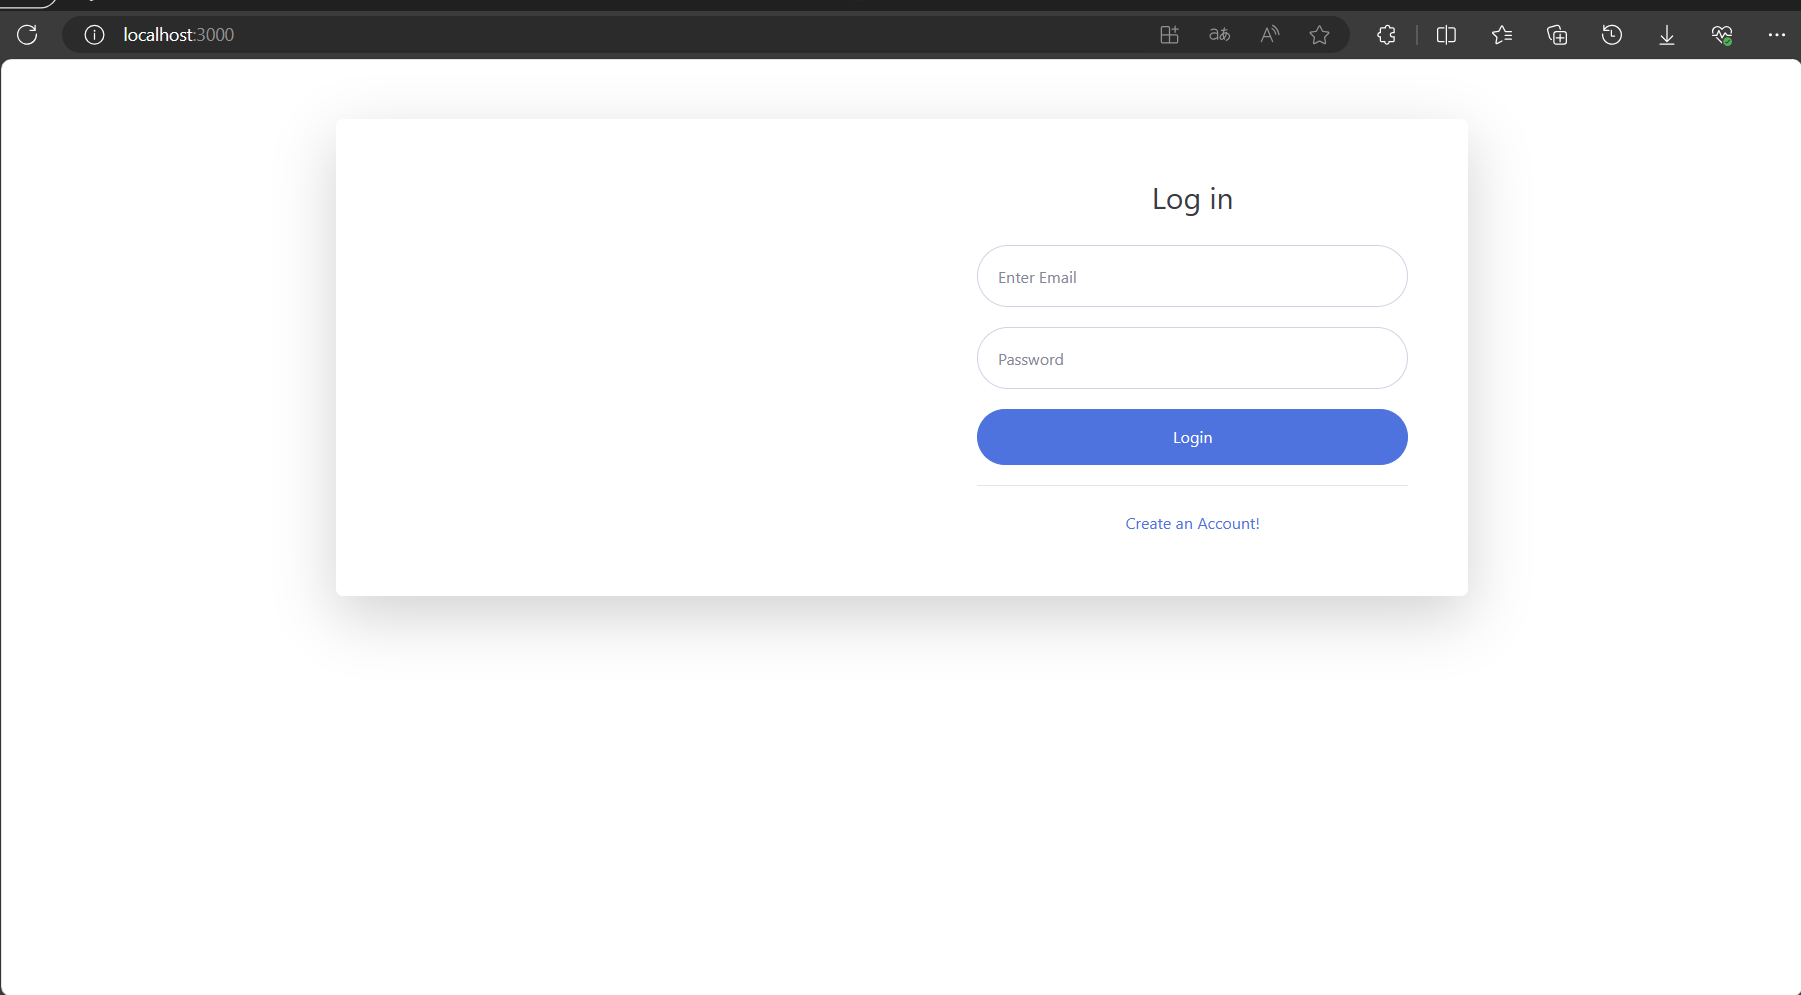
\includegraphics[scale=0.3]{login.png}
  \caption[หน้า Login]{หน้า Login}
  \label{fig:login}
\end{figure}

\subsubsection{Register page} 
\enskip \enskip \enskip \enskip \enskip
ผู้ใช้ที่ยังไม่ได้ทำการสมัครกับทางเรา สามารถสมัครกับทางเราได้โดยการกรอกข้อมูล ชื่อจริง-นามสกุลอีเมล์และรหัสผ่าน
\graphicspath{ {./images/} }
\begin{figure}[htbp]
  \centering 
  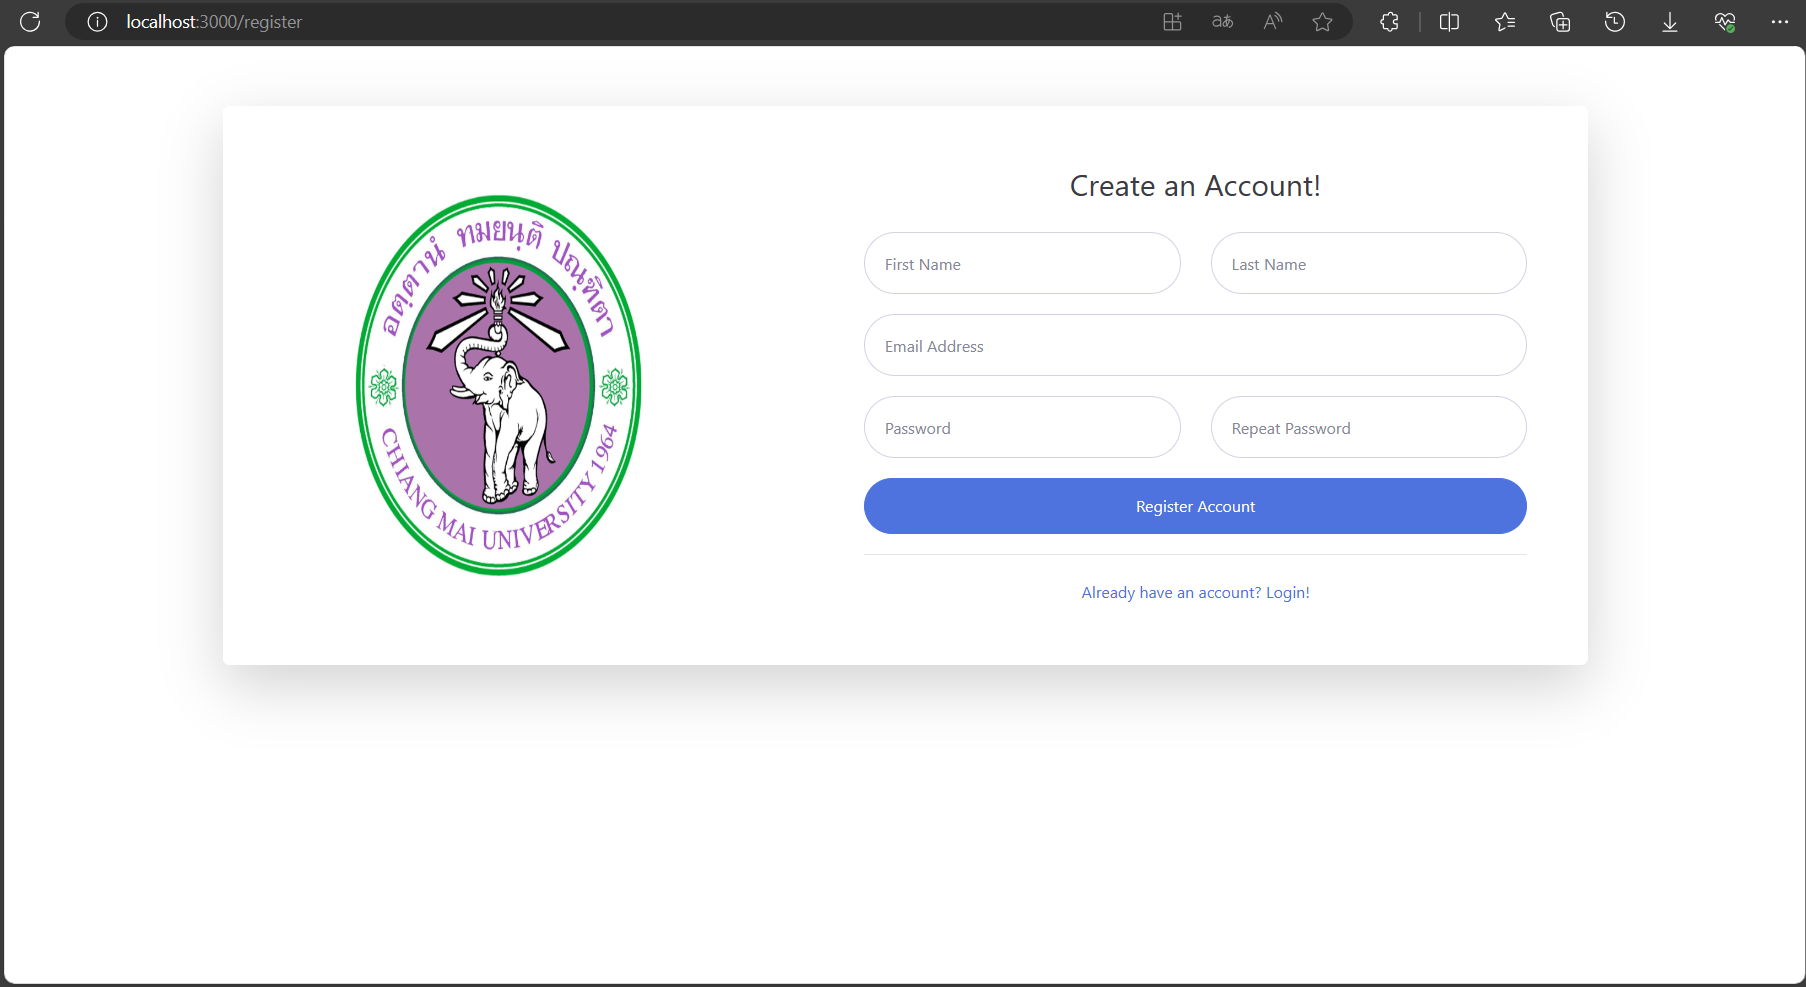
\includegraphics[scale=0.3]{register.png}
  \caption[หน้า Register]{หน้า Register}
  \label{fig:Register}
\end{figure}
\\\\\\
\subsubsection{Otp-Verification page} 
\enskip \enskip \enskip \enskip \enskip
หลังจากผู้ใช้ทำการกรอกข้อมูลสมัครกับทางเราแล้วทางเราจะส่ง OTP เพื่อยืนยันตัวตนของผู้ใช้ให้ผู้ใช้นำ OTP ที่ได้รับนำมากรอกในหน้านี้
\graphicspath{ {./images/} }
\begin{figure}[htbp]
  \centering 
  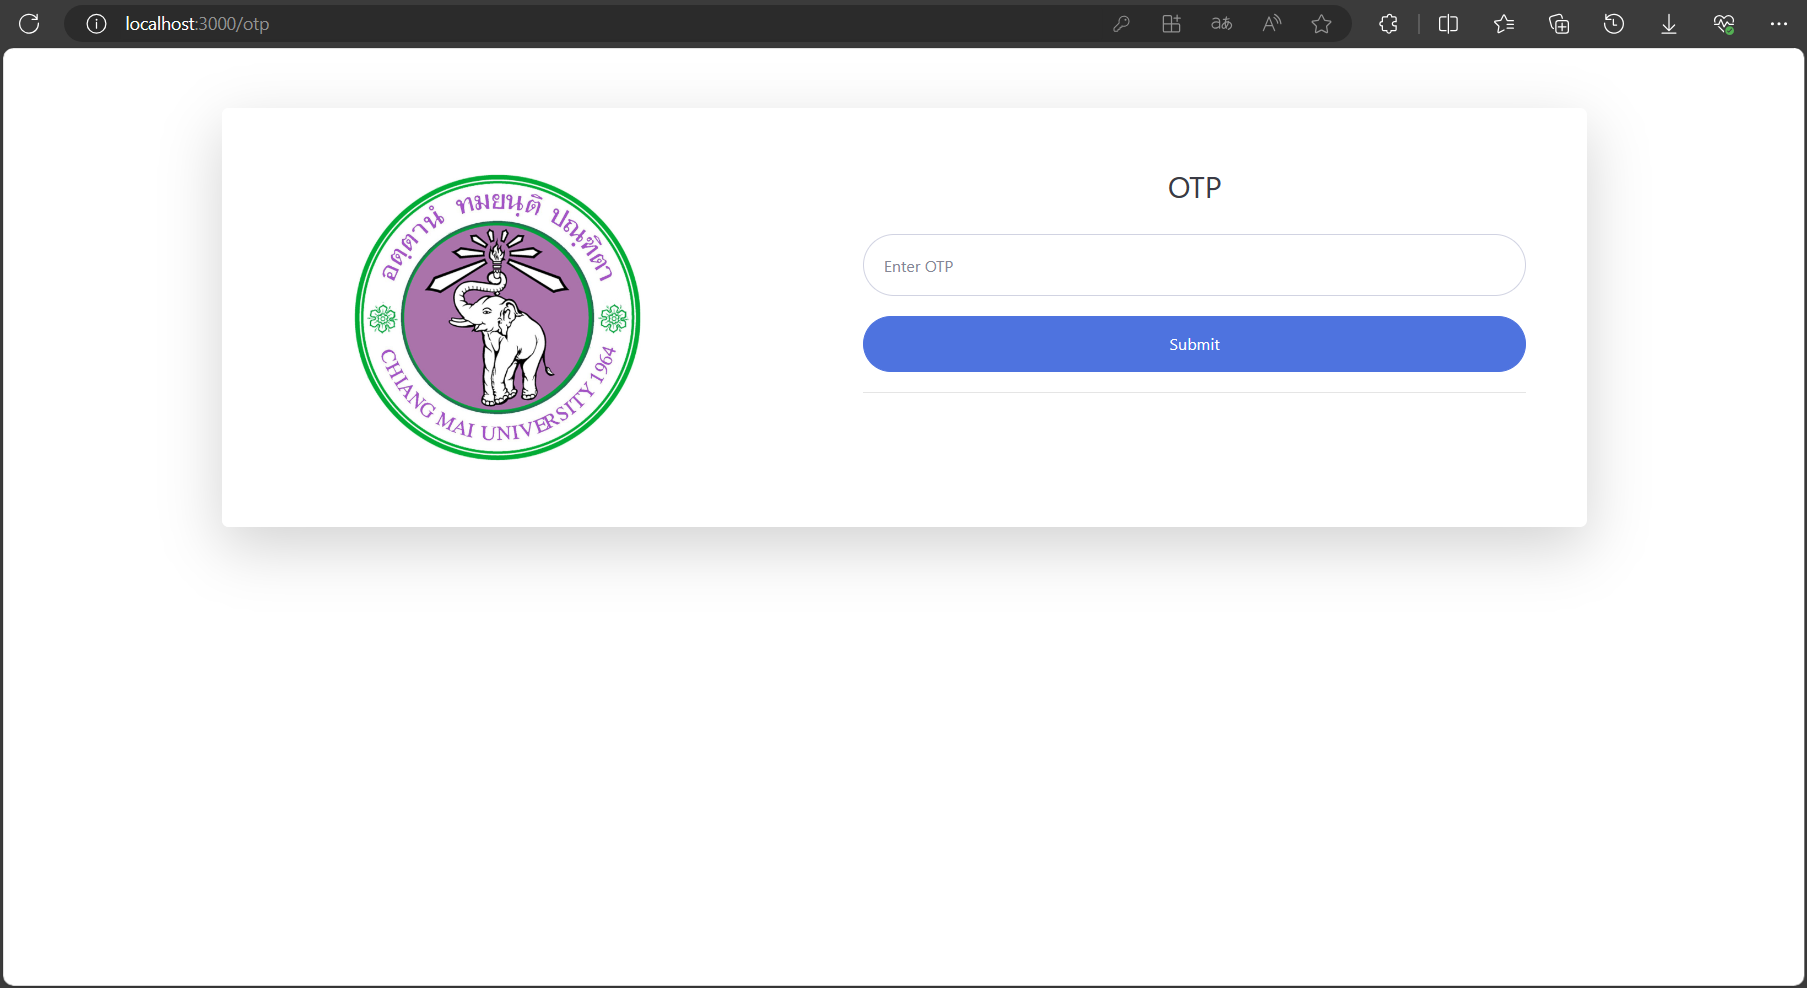
\includegraphics[scale=0.3]{otp.png}
  \caption[หน้ากรอกยืนยัน OTP]{หน้ากรอกยืนยัน OTP}
  \label{fig:Otp}
\end{figure}

\subsubsection{Dash-Board page} 
\enskip \enskip \enskip \enskip \enskip
ในหน้านี้จะแสดงข้อมูลต่างๆ บอกอยู่ อาทิ ข้อมูลใบประกาศนียบัตรที่สร้างไปแล้ว ข้อมูลใบประกาศนียบัตรที่ยังสร้างไม่เสร็จ และ มีระบบ quick create ที่สามารถสร้างใบประกาศนียบัตรอย่างรวดเร็ว และมีเมนูให้เลือกสองเมนู คือ 
\begin{enumerate}
  \item สร้างใบประกาศนียบัตรสำหรับหนึ่งคน
  \item สร้างใบประกาศนียบัตรสำหรับหนึ่งคอร์สเรียน
  \end{enumerate}
\graphicspath{ {./images/} }
\begin{figure}[htbp]
  \centering 
  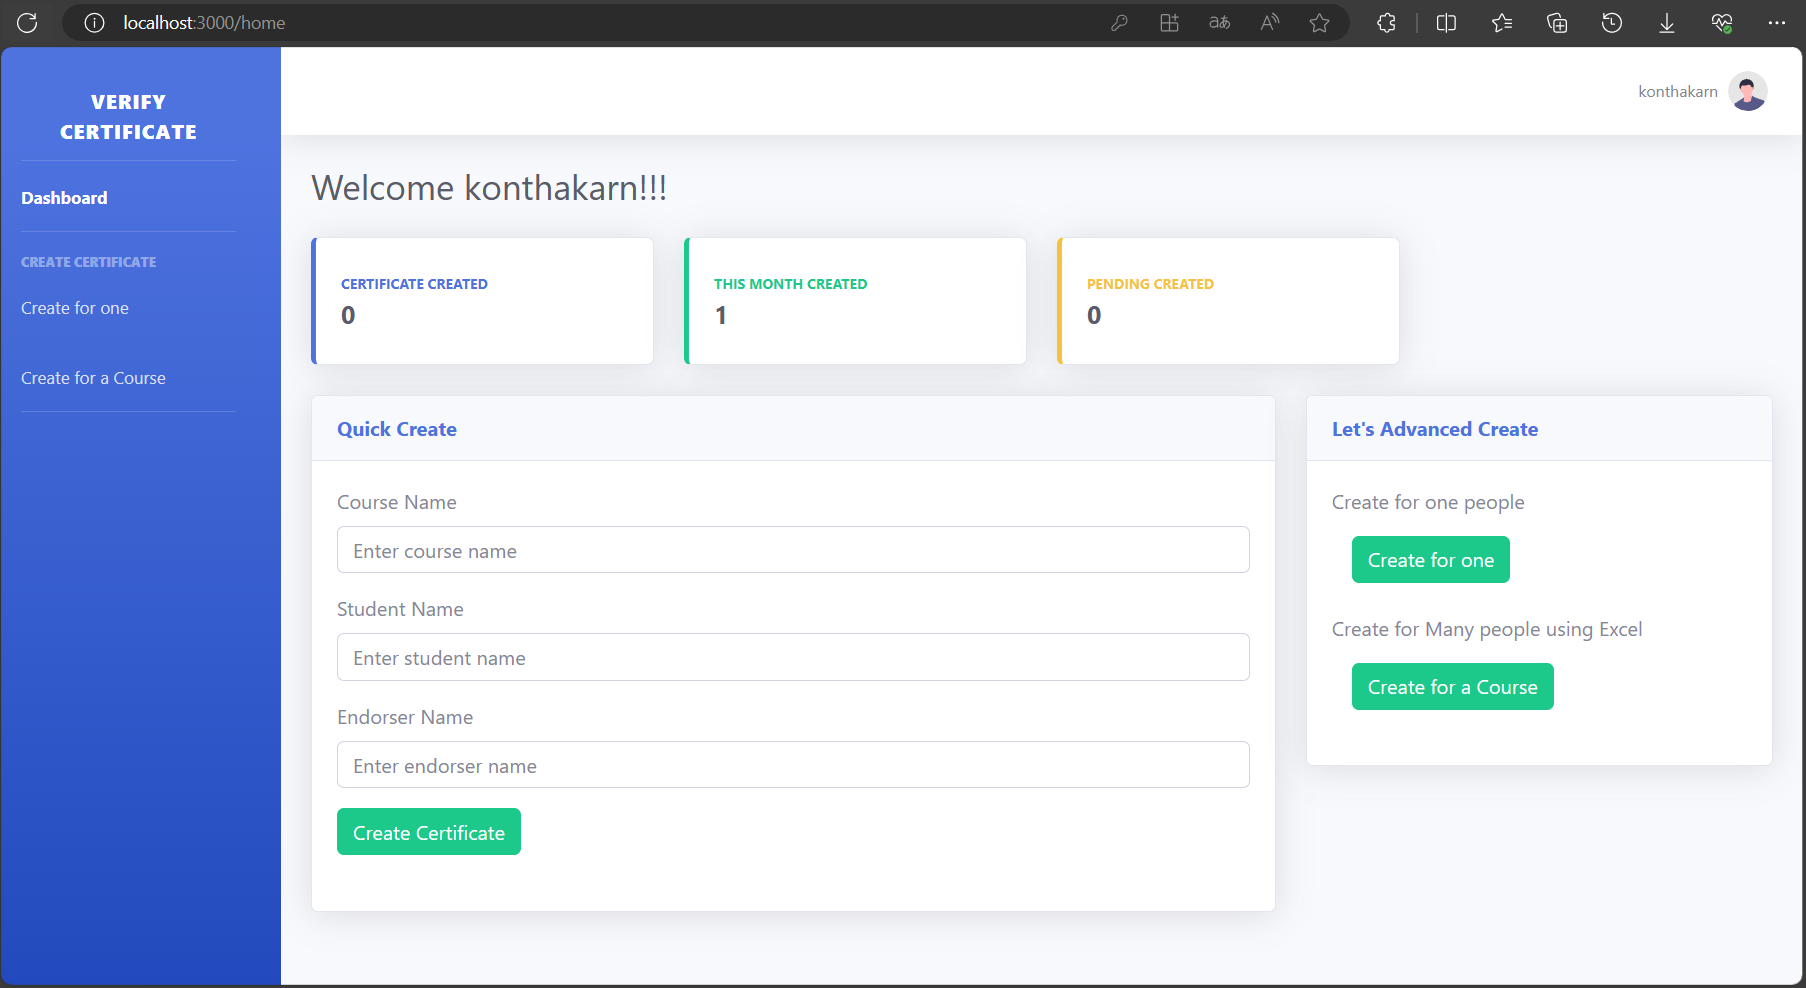
\includegraphics[scale=0.3]{dash.png}
  \caption[หน้า Dash-Board]{หน้า Dash-Board}
  \label{fig:Dash-Board}
\end{figure}

\subsubsection{Create For One page} 
\enskip \enskip \enskip \enskip \enskip
เมื่อเรากดcreate for one ระบบจะนำมายังหน้านี้ ในหน้านี้จะเป็นหน้าสำหรับสร้างใบประกาศนียบัตรสำหรับหนึ่งคนผู้ใช้จะทำการกรอกข้อมูลต่างๆในฟอร์มเพื่อทำการสร้างใบประกาศนียบัตร
\graphicspath{ {./images/} }
\begin{figure}[htbp]
  \centering 
  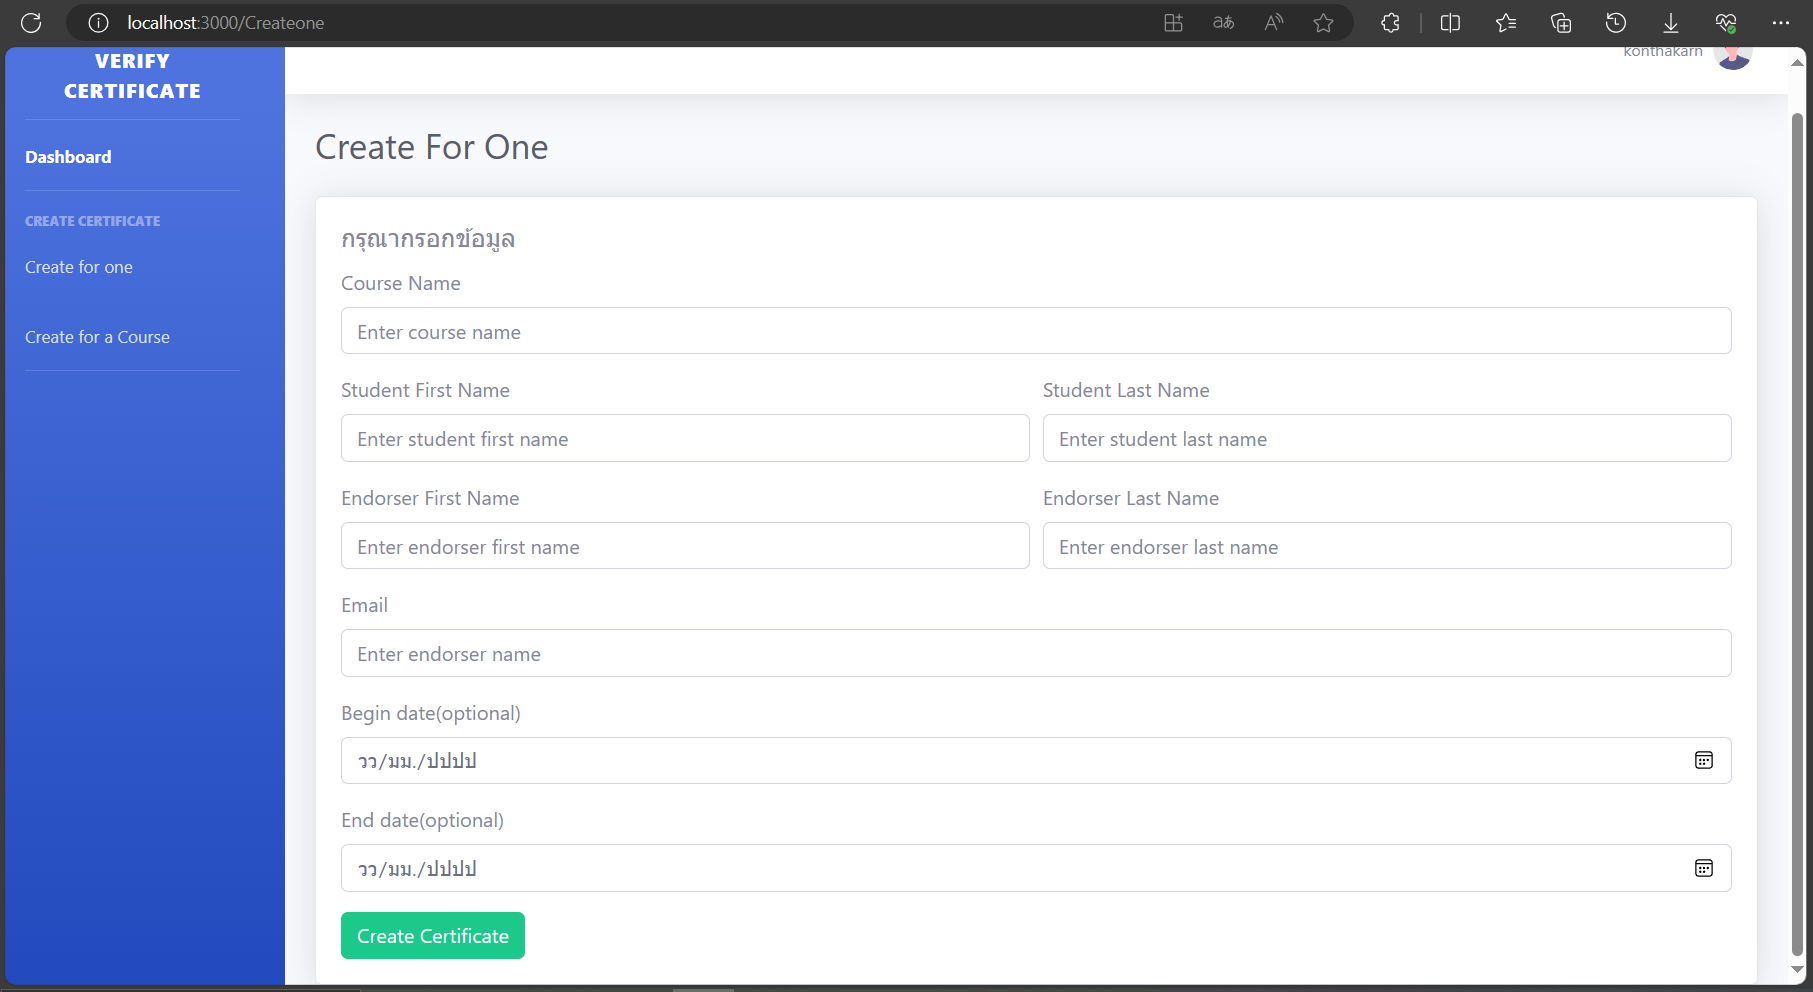
\includegraphics[scale=0.3]{creone.png}
  \caption[หน้า Create For One]{หน้า Create For One}
  \label{fig:Create For One}
\end{figure}

\subsubsection{Create For Course page} 
\enskip \enskip \enskip \enskip \enskip
เมื่อเรากดCreate for course จะนำมายังหน้านี้ ในส่วนนี้จะแสดงตารางคอร์สต่างๆที่เราเคยสร้างไว้และจะมีกดปุ่มเพื่อสร้างคอร์สใหม่ และกดปุ่มเพื่อทำการอิมพอร์ตข้อมูลเพื่อออกใบประกาศนียบัตร
\graphicspath{ {./images/} }
\begin{figure}[htbp]
  \centering 
  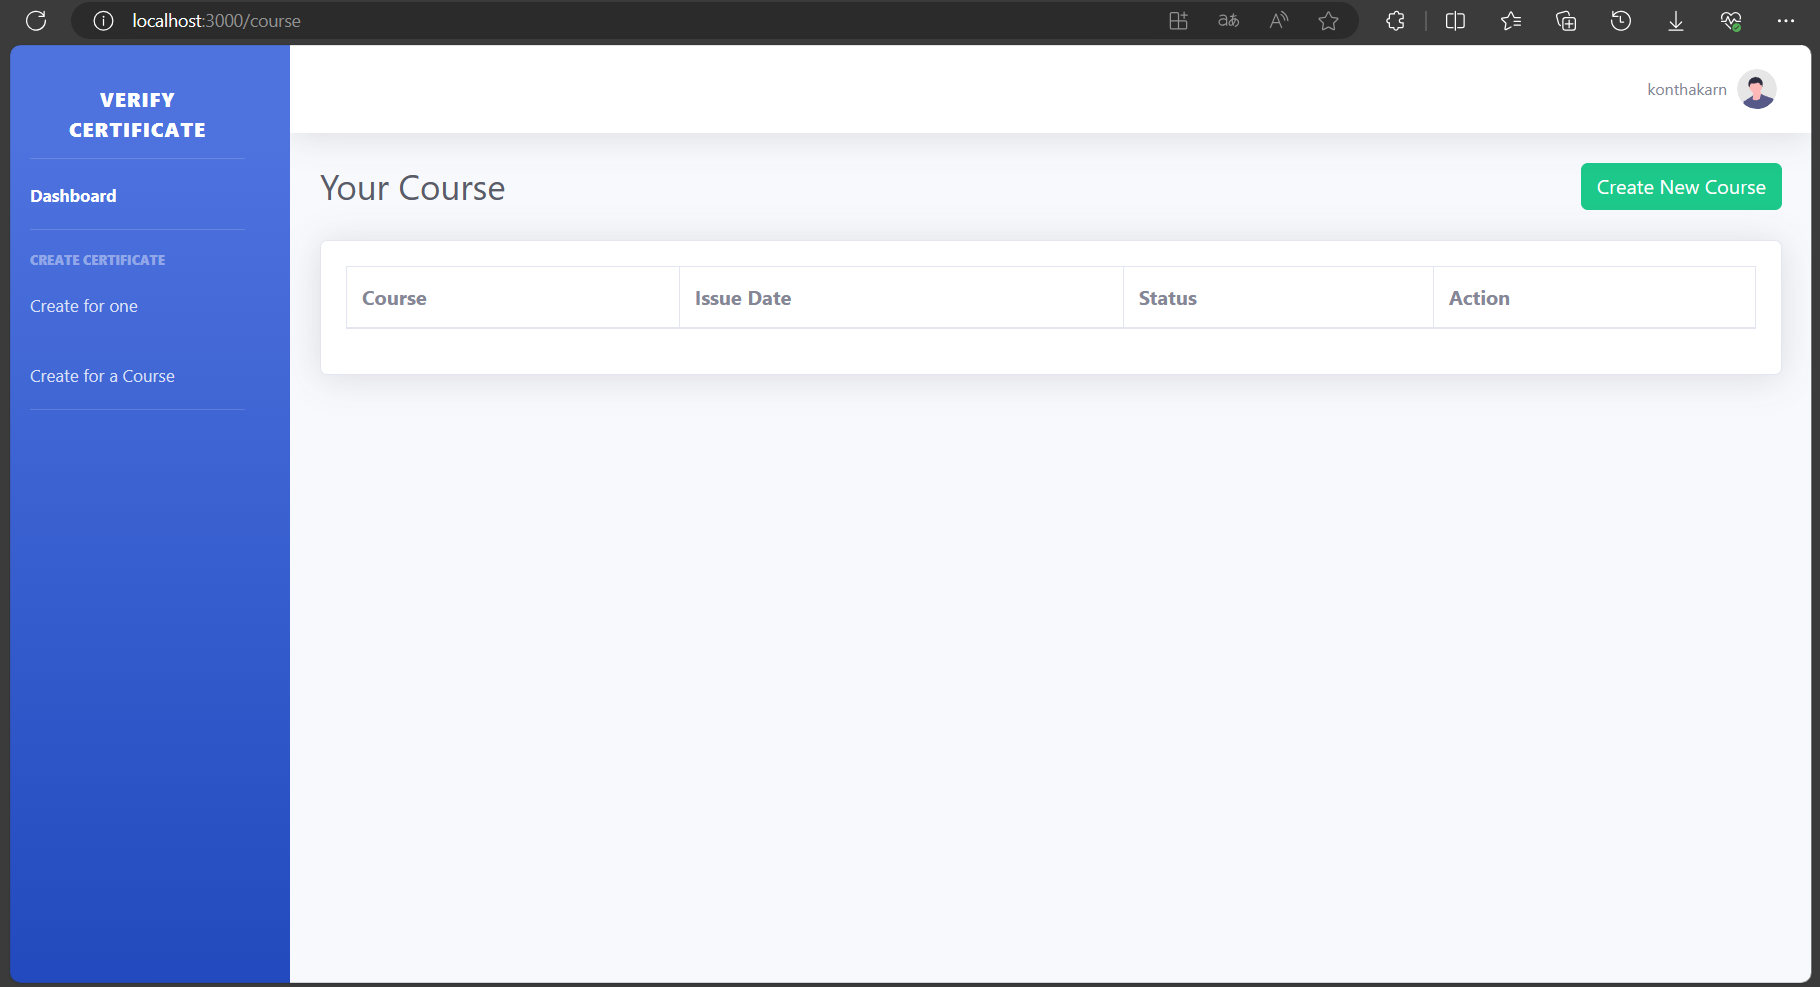
\includegraphics[scale=0.3]{crec.png}
  \caption[หน้า Create For Course]{หน้า Create For Course}
  \label{fig:Create For Course}
\end{figure}
\\\\\\\\
\subsubsection{Export To Excel page} 
\enskip \enskip \enskip \enskip \enskip
เมื่อเรากดปุ่มอิมพอร์ตข้อมูลในหน้า Create For Course page ระบบจะนำมายังหน้านี้ในส่วนนี้จะมีปุ่มให้กด Export ไฟล์ Excel ที่เรา Config หัวข้อที่ผู้ใช้เลือกไว้สำหรับให้ผู้ใช้กรอกข้อมูลต่างๆตามหัวข้อที่ เลือกไว้แล้วนำมาอัพโหลดเพื่อสร้างใบประกาศนียบัตรในขั้นตอนต่อไป 
\graphicspath{ {./images/} }
\begin{figure}[htbp]
  \centering 
  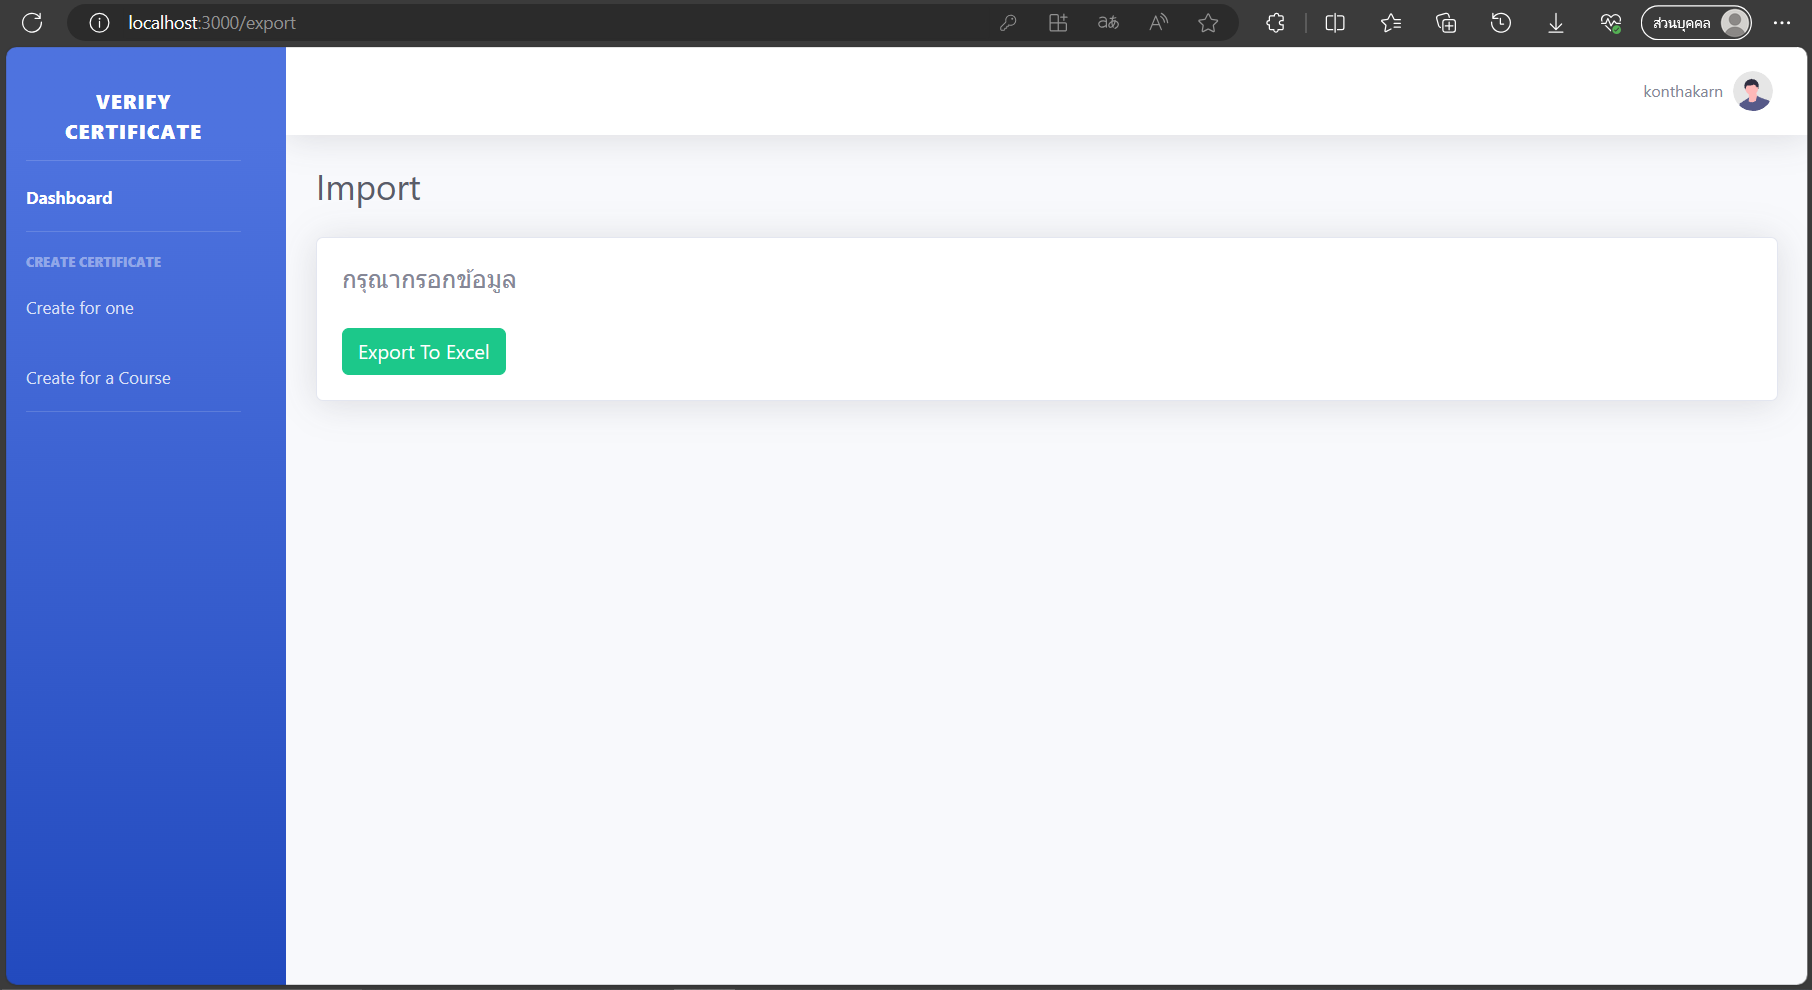
\includegraphics[scale=0.3]{excel.png}
  \caption[หน้า Export To Excel]{หน้า Export To Excel}
  \label{fig:Export To Excel}
\end{figure}

\subsubsection{Import Excel page} 
\enskip \enskip \enskip \enskip \enskip
พอเรากรอกข้อมูลลงใน Excel เสร็จแล้วระบบจะมีหน้าให้อัพโหลดไฟล์เข้าไปเพื่อทำการสร้างใบ ประกาศนียบัตรพอเราอัพโหลดไฟล์ Excel เสร็จเรียบร้อยระบบจะทำการ generate ใบประกาศนียบัตร และทำการ ส่งemailพร้อมใบประกาศนียบัตรให้ผู้รับอัตโนมัติและสามารถตรวจสอบใบประกาศนียบัตรที่สร้างได้
\graphicspath{ {./images/} }
\begin{figure}[htbp]
  \centering 
  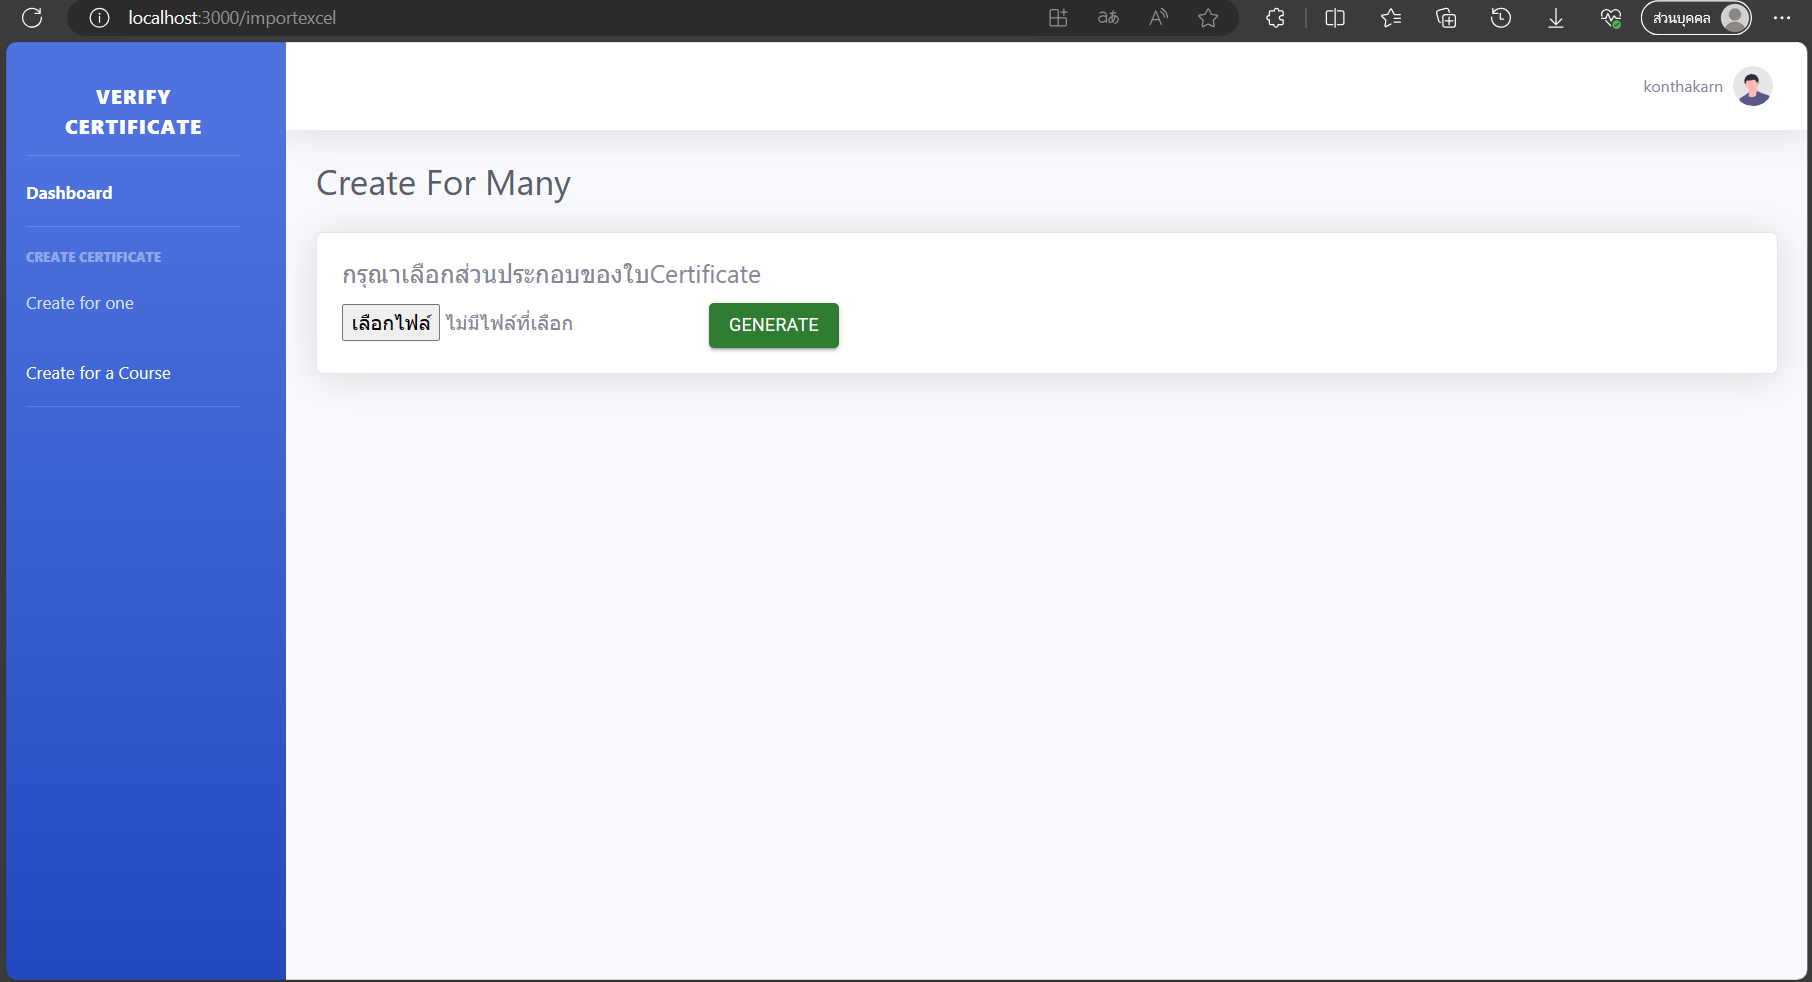
\includegraphics[scale=0.3]{excel2.png}
  \caption[หน้า Import Excel page]{หน้า Import Excel page}
  \label{fig:Import Excel page}
\end{figure}

\subsubsection{View Course page} 
\enskip \enskip \enskip \enskip \enskip
ในหน้านี้จะแสดงข้อมูลเกี่ยงกับนักเรียนที่เรียนในคอร์สและสามารถดาวน์โหลดใบประกาศนียบัตรของนักเรียนคนไหนก็ได้
\graphicspath{ {./images/} }
\begin{figure}[htbp]
  \centering 
  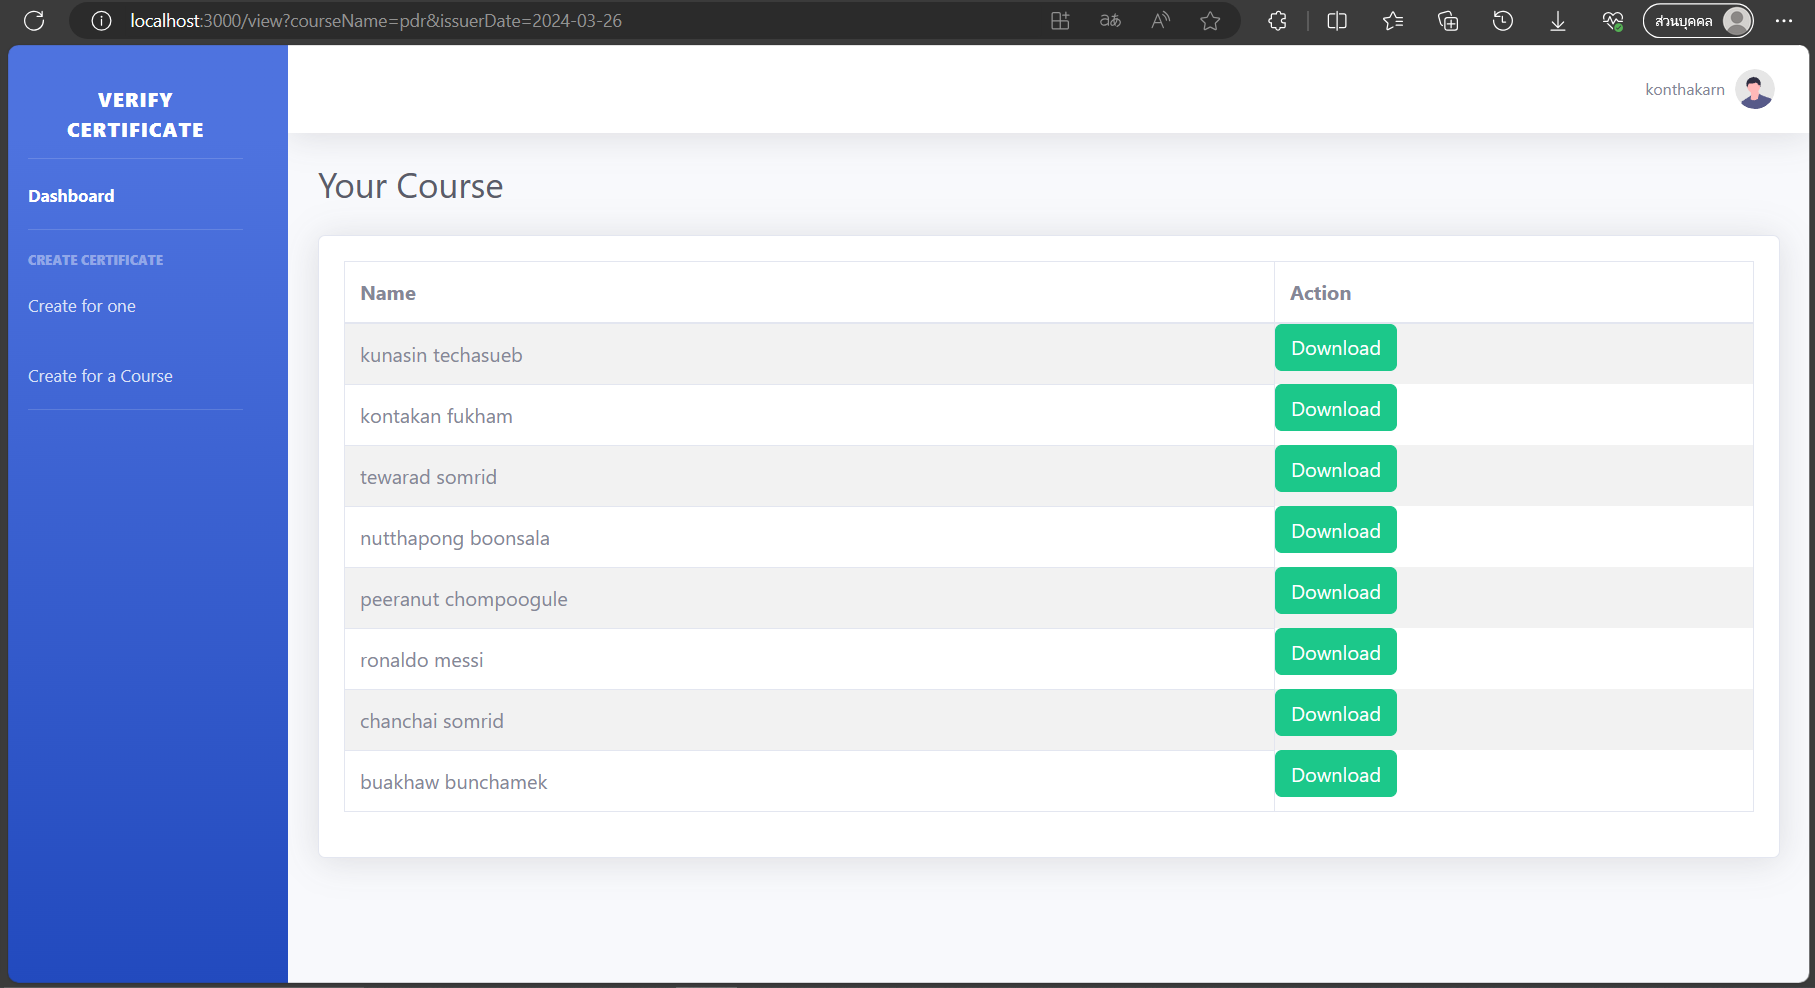
\includegraphics[scale=0.3]{view.png}
  \caption[หน้า View Course page]{หน้า View Course page}
  \label{fig:View Course page}
\end{figure}

\subsection{ผู้ที่ต้องการจะตรวจสอบใบcertificate}
\enskip \enskip \enskip \enskip \enskip
ในส่วนนี้ผู้ใช้สามารถแสกน QR Code ที่อยู่ในใบประกาศนียบัตรแล้วจะนำพาไปยังลิ้งที่ขึ้นรูปภาพของใบประกาศนียบัตรนั้นให้ผู้ใช้งานตรวจสอบความถูกต้อง จะเก็บข้อมูลของใบประกาศนียบัตรตามรูป
\graphicspath{ {./images/} }
\begin{figure}[htbp]
  \centering 
  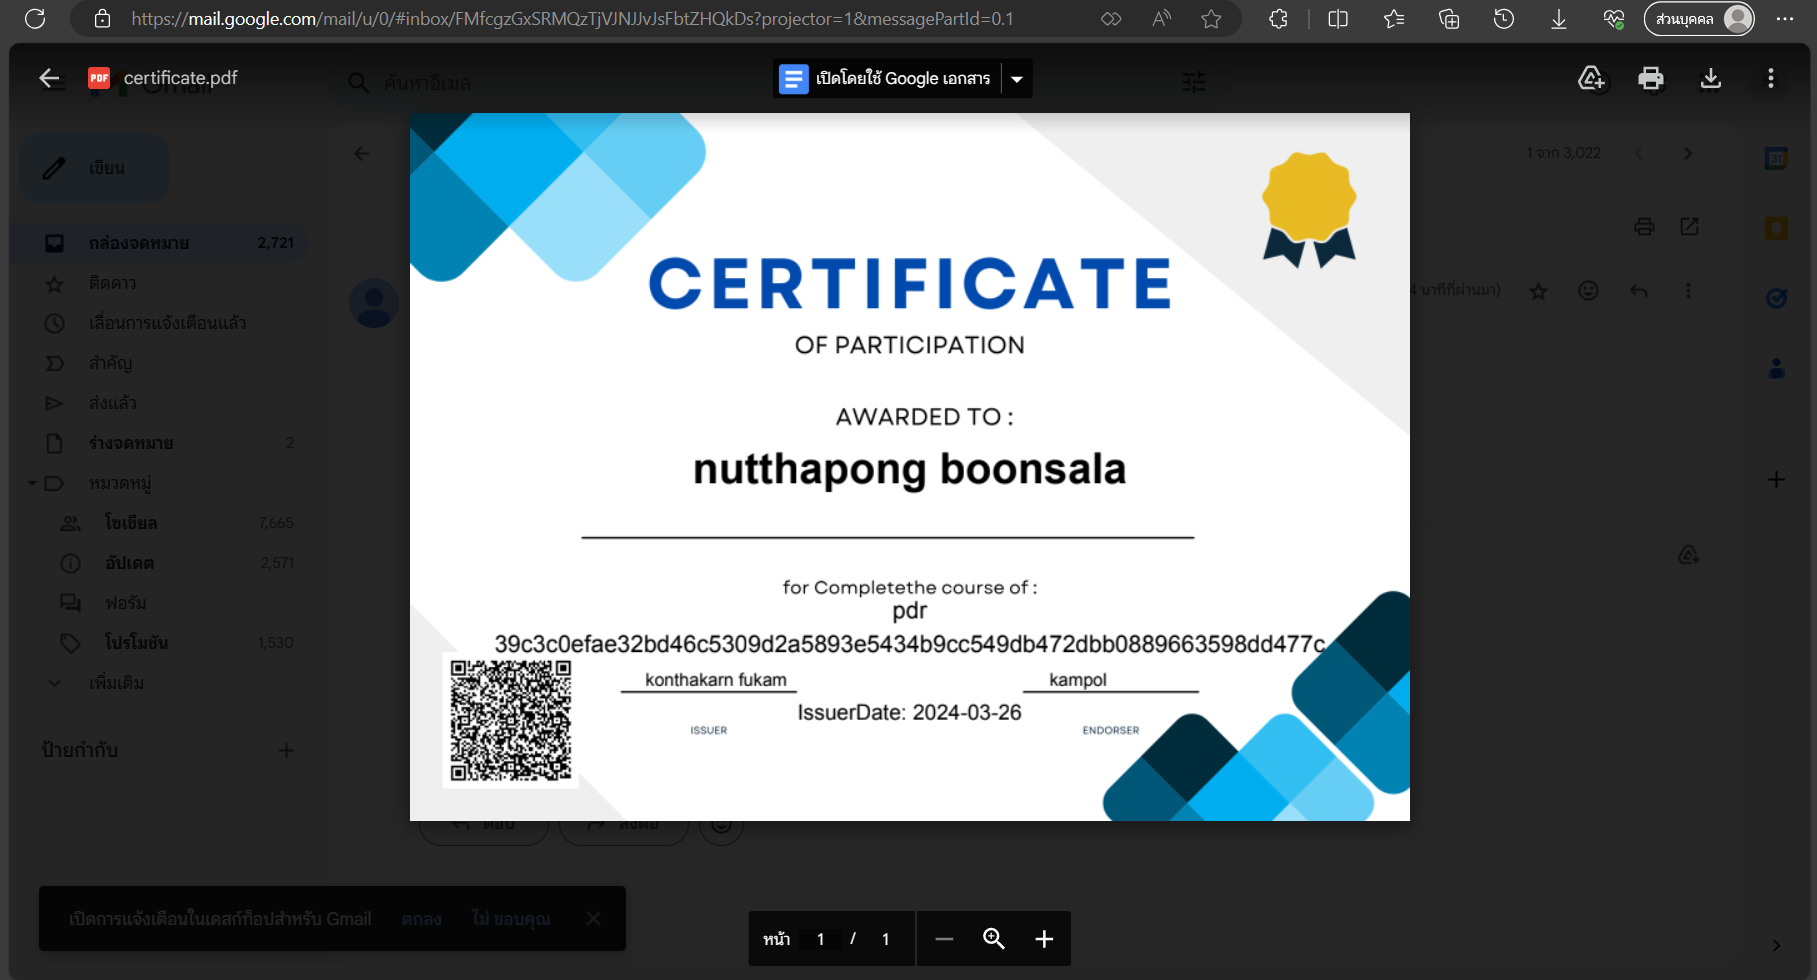
\includegraphics[scale=0.3]{cer.png}
  \caption[หน้าใบประกาศนียบัตร]{หน้าใบประกาศนียบัตร}
  \label{fig:PPPPPPP}
\end{figure}